\subsection{x86: 3 arguments}

\subsubsection{MSVC}

When we compile it with MSVC 2010 Express we get:

\begin{lstlisting}
$SG3830	DB	'a=%d; b=%d; c=%d', 00H

...

	push	3
	push	2
	push	1
	push	OFFSET $SG3830
	call	_printf
	add	esp, 16					; 00000010H
\end{lstlisting}

Almost the same, but now we can see the \printf arguments are pushed onto the stack in reverse order. The first argument is pushed last.

By the way, variables of \Tint type in 32-bit environment have 32-bit width, that is 4 bytes.

So, we have 4 arguments here. $4*4 = 16$~---they occupy exactly 16 bytes in the stack: a 32-bit pointer to a string and 3 numbers of type \Tint.

\index{x86!\Instructions!ADD}
\index{x86!\Registers!ESP}
\index{cdecl}
When the \gls{stack pointer} (\ESP register) has changed back by the \INS{ADD ESP, X}
instruction after a function 
call, often, the number of function arguments could be deduced by simply dividing X by 4.

Of course, this is specific to the \IT{cdecl} calling convention, and only for 32-bit environment.

\ifx\LITE\undefined
See also the calling conventions section ~(\myref{sec:callingconventions}).
\fi

In certain cases where several functions return right after one another, the compiler could merge multiple \q{ADD ESP, X} instructions into one, after the last call:

\begin{lstlisting}
push a1
push a2
call ...
...
push a1
call ...
...
push a1
push a2
push a3
call ...
add esp, 24
\end{lstlisting}

Here is a real-world example:

\lstinputlisting[caption=x86]{patterns/03_printf/x86/add_example.lst.\LANG}

\ifdefined\IncludeOlly
\clearpage
\subsubsection{MSVC and \olly}
\index{\olly}

Now let's try to load this example in \olly.
It is one of the most popular user-land win32 debuggers.
We can compile our example in MSVC 2012 with \GTT{/MD} option, which means to link with \GTT{MSVCR*.DLL},
so we can see the imported functions clearly in the debugger.

Then load the executable in \olly.
The very first breakpoint is in \GTT{ntdll.dll}, press 
F9 (run).
The second breakpoint is in \ac{CRT}-code.
Now we have to find the \main function.

Find this code by scrolling the code to the very top (MSVC allocates the \main function at the very beginning of the code section): 
\begin{figure}[H]
\centering
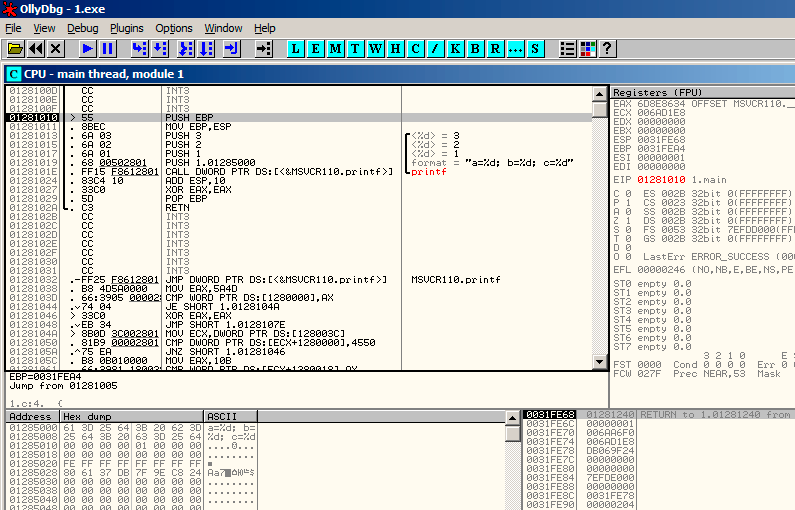
\includegraphics[scale=\FigScale]{patterns/03_printf/x86/olly3_1.png}
\caption{\olly: the very start of the \main function}
\label{fig:printf3_olly_1}
\end{figure}

Click on the \INS{PUSH EBP} instruction, press F2 (set breakpoint) and press F9 (run).
We need to perform these actions in order to skip \ac{CRT}-code, because we aren't really interested in it yet.

\clearpage
Press F8 (\stepover) 6 times, i.e. skip 6 instructions:

\begin{figure}[H]
\centering
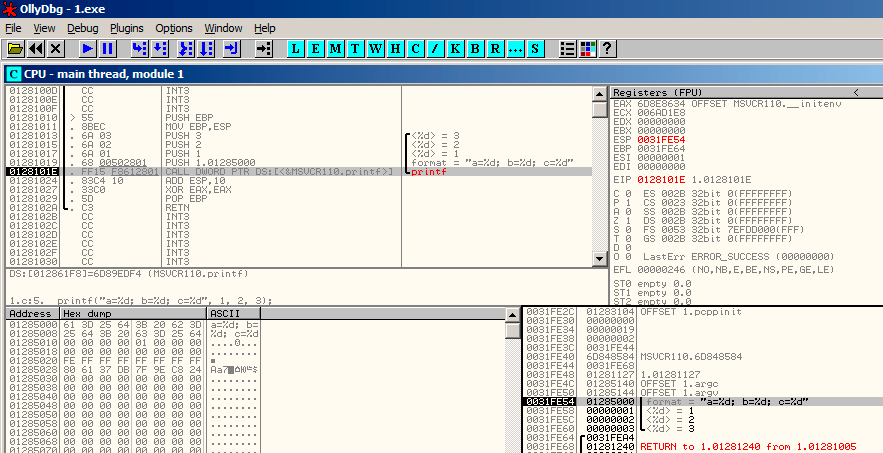
\includegraphics[scale=\FigScale]{patterns/03_printf/x86/olly3_2.png}
\caption{\olly: before \printf execution}
\label{fig:printf3_olly_2}
\end{figure}

Now the \ac{PC} points to the \INS{CALL printf} instruction.
\olly, like other debuggers, highlights the value of the registers which were changed.
So each time you press F8, \EIP changes and its value is displayed in red.
\ESP changes as well, because the arguments values are pushed into the stack.\\
\\
Where are the values in the stack?
Take a look at the right bottom debugger window:

\begin{figure}[H]
\centering
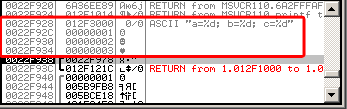
\includegraphics[scale=\NormalScale]{patterns/03_printf/x86/olly3_stack.png}
\caption{\olly: stack after the argument values have been pushed (The red rectangular border was added by me in a graphics editor)}
\end{figure}

We can see 3 columns there: address in the stack, value in the stack and some additional \olly comments. 
\olly understands \printf{}-like strings, so it reports the string here and the 3 values \IT{attached} to it.

It is possible to right-click on the format string, click on \q{Follow in dump},
and the format string will appear in the debugger left-bottom window, which always displays some part of the memory.
These memory values can be edited.
It is possible to change the format string, in which case the result of our example would be different.
It is not very useful in this particular case, but it could be good as an exercise so you start building a feel of how everything works here.

\clearpage
Press F8 (\stepover).

We see the following output in the console:

\begin{figure}[H]
\centering
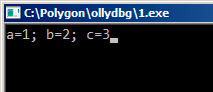
\includegraphics[scale=\NormalScale]{patterns/03_printf/x86/olly3_console.png}
\caption{\printf function executed}
\end{figure}

Let's see how the registers and stack state have changed: 

\begin{figure}[H]
\centering
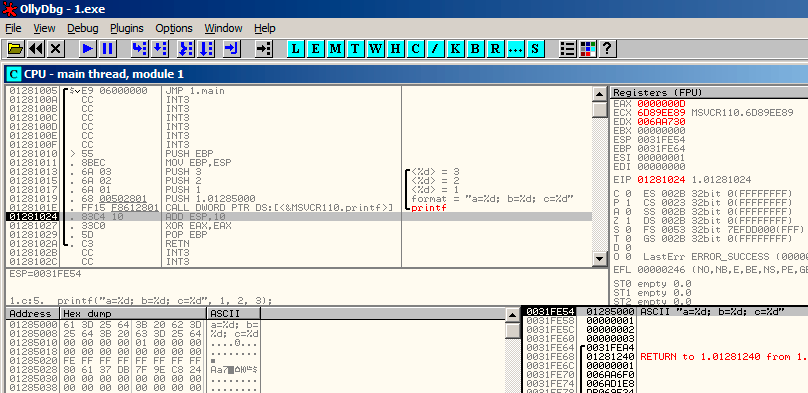
\includegraphics[scale=\FigScale]{patterns/03_printf/x86/olly3_3.png}
\caption{\olly after \printf{} execution}
\label{fig:printf3_olly_3}
\end{figure}

Register \EAX now contains \GTT{0xD} (13).
That is correct, since \printf returns the number of characters printed. 
The value of \EIP has changed: indeed, now it contains the address of the instruction coming after 
\INS{CALL printf}.
\ECX and \EDX values have changed as well.
Apparently, the \printf function's hidden machinery used them for its own needs.

A very important fact is that neither the \ESP value, nor the stack state have been changed!
We clearly see that the format string and corresponding 3 values are still there.
This is indeed the \IT{cdecl} calling convention behaviour: \gls{callee} does not return \ESP back to its previous value.
The \gls{caller} is responsible to do so.

\clearpage
Press F8 again to execute \INS{ADD ESP, 10} instruction:

\begin{figure}[H]
\centering
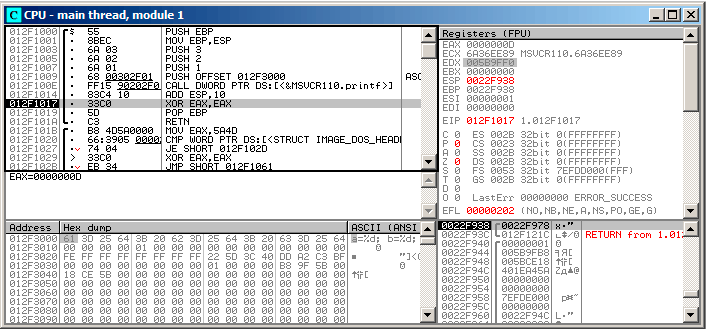
\includegraphics[scale=\FigScale]{patterns/03_printf/x86/olly3_4.png}
\caption{\olly: after \INS{ADD ESP, 10} instruction execution}
\label{fig:printf3_olly_4}
\end{figure}

\ESP has changed, but the values are still in the stack!
Yes, of course; no one needs to set these values to zeroes or something like that.
Everything above the stack pointer (\ac{SP}) 
is \IT{noise} or \IT{\garbage{}} and has no meaning at all.
It would be time consuming to clear the unused stack entries anyway, and no one really needs to.

\fi % IncludeOlly

\ifdefined\IncludeGCC
\subsubsection{GCC}

Now let's compile the same program in Linux using GCC 4.4.1 and take a look at what we have got in \IDA:

\begin{lstlisting}
main            proc near

var_10          = dword ptr -10h
var_C           = dword ptr -0Ch
var_8           = dword ptr -8
var_4           = dword ptr -4

                push    ebp
                mov     ebp, esp
                and     esp, 0FFFFFFF0h
                sub     esp, 10h
                mov     eax, offset aADBDCD ; "a=%d; b=%d; c=%d"
                mov     [esp+10h+var_4], 3
                mov     [esp+10h+var_8], 2
                mov     [esp+10h+var_C], 1
                mov     [esp+10h+var_10], eax
                call    _printf
                mov     eax, 0
                leave
                retn
main            endp
\end{lstlisting}

Its noticeable that the difference between the MSVC code and the GCC code is only in the way the arguments are stored on the stack.
Here the GCC is working directly with the stack without the use of \PUSH/\POP.

\ifdefined\IncludeGDB
\subsubsection{GCC and GDB}
\index{GDB}

Let's try this example also in \ac{GDB} in Linux.

\GTT{-g} option instructs the compiler to include debug information in the executable file.

\begin{lstlisting}
$ gcc 1.c -g -o 1
\end{lstlisting}

\begin{lstlisting}
$ gdb 1
GNU gdb (GDB) 7.6.1-ubuntu
Copyright (C) 2013 Free Software Foundation, Inc.
License GPLv3+: GNU GPL version 3 or later <http://gnu.org/licenses/gpl.html>
This is free software: you are free to change and redistribute it.
There is NO WARRANTY, to the extent permitted by law.  Type "show copying"
and "show warranty" for details.
This GDB was configured as "i686-linux-gnu".
For bug reporting instructions, please see:
<http://www.gnu.org/software/gdb/bugs/>...
Reading symbols from /home/dennis/polygon/1...done.
\end{lstlisting}

\begin{lstlisting}[caption=let's set breakpoint on \printf]
(gdb) b printf
Breakpoint 1 at 0x80482f0
\end{lstlisting}

Run.
We don't have the \printf function source code here, so \ac{GDB} can't show it, but may do so.

\begin{lstlisting}
(gdb) run
Starting program: /home/dennis/polygon/1 

Breakpoint 1, __printf (format=0x80484f0 "a=%d; b=%d; c=%d") at printf.c:29
29	printf.c: No such file or directory.
\end{lstlisting}

Print 10 stack elements. The most left column contains addresses on the stack.

\begin{lstlisting}
(gdb) x/10w $esp
0xbffff11c:	0x0804844a	0x080484f0	0x00000001	0x00000002
0xbffff12c:	0x00000003	0x08048460	0x00000000	0x00000000
0xbffff13c:	0xb7e29905	0x00000001
\end{lstlisting}

The very first element is the \ac{RA} (\GTT{0x0804844a}).
We can verify this by disassembling the memory at this address:

\begin{lstlisting}[label=NOP_as_XCHG_example]
(gdb) x/5i 0x0804844a
   0x804844a <main+45>:	mov    $0x0,%eax
   0x804844f <main+50>:	leave  
   0x8048450 <main+51>:	ret    
   0x8048451:	xchg   %ax,%ax
   0x8048453:	xchg   %ax,%ax
\end{lstlisting}

The two \INS{XCHG} instructions are idle instructions, analogous to \ac{NOP}s.

The second element (\GTT{0x080484f0}) is the format string address:

\begin{lstlisting}
(gdb) x/s 0x080484f0
0x80484f0:	"a=%d; b=%d; c=%d"
\end{lstlisting}

Next 3 elements (1, 2, 3) are the \printf arguments.
The rest of the elements could be just \q{garbage} on the stack, 
but could also be values from other functions, their local variables, \etc{}.
We can ignore them for now.

Run \q{finish}. 
The command instructs GDB to \q{execute all instructions until the end of the function}.
In this case: execute till the end of \printf.

\begin{lstlisting}
(gdb) finish
Run till exit from #0  __printf (format=0x80484f0 "a=%d; b=%d; c=%d") at printf.c:29
main () at 1.c:6
6		return 0;
Value returned is $2 = 13
\end{lstlisting}

\ac{GDB} shows what \printf returned in \EAX (13).
This is the number of characters printed out, just like in the \olly example.

We also see \q{return 0;} and the information that this expression is in the \GTT{1.c} file at the line 6.
Indeed, the \GTT{1.c} file is located in the current directory, and \ac{GDB} finds the string there.
How does \ac{GDB} know which C-code line is being currently executed?
This is due to the fact that the compiler,
while generating debugging information, also saves a table of relations between source code line
numbers and instruction addresses.
GDB is a source-level debugger, after all.

Let's examine the registers.
13 in \EAX:

\begin{lstlisting}
(gdb) info registers
eax            0xd	13
ecx            0x0	0
edx            0x0	0
ebx            0xb7fc0000	-1208221696
esp            0xbffff120	0xbffff120
ebp            0xbffff138	0xbffff138
esi            0x0	0
edi            0x0	0
eip            0x804844a	0x804844a <main+45>
...
\end{lstlisting}

Let's disassemble the current instructions.
The arrow points to the instruction to be executed next.

\begin{lstlisting}
(gdb) disas
Dump of assembler code for function main:
   0x0804841d <+0>:	push   %ebp
   0x0804841e <+1>:	mov    %esp,%ebp
   0x08048420 <+3>:	and    $0xfffffff0,%esp
   0x08048423 <+6>:	sub    $0x10,%esp
   0x08048426 <+9>:	movl   $0x3,0xc(%esp)
   0x0804842e <+17>:	movl   $0x2,0x8(%esp)
   0x08048436 <+25>:	movl   $0x1,0x4(%esp)
   0x0804843e <+33>:	movl   $0x80484f0,(%esp)
   0x08048445 <+40>:	call   0x80482f0 <printf@plt>
=> 0x0804844a <+45>:	mov    $0x0,%eax
   0x0804844f <+50>:	leave  
   0x08048450 <+51>:	ret    
End of assembler dump.
\end{lstlisting}

\ac{GDB} uses AT\&T syntax by default.
But it is possible to switch to Intel syntax:

\begin{lstlisting}
(gdb) set disassembly-flavor intel
(gdb) disas
Dump of assembler code for function main:
   0x0804841d <+0>:	push   ebp
   0x0804841e <+1>:	mov    ebp,esp
   0x08048420 <+3>:	and    esp,0xfffffff0
   0x08048423 <+6>:	sub    esp,0x10
   0x08048426 <+9>:	mov    DWORD PTR [esp+0xc],0x3
   0x0804842e <+17>:	mov    DWORD PTR [esp+0x8],0x2
   0x08048436 <+25>:	mov    DWORD PTR [esp+0x4],0x1
   0x0804843e <+33>:	mov    DWORD PTR [esp],0x80484f0
   0x08048445 <+40>:	call   0x80482f0 <printf@plt>
=> 0x0804844a <+45>:	mov    eax,0x0
   0x0804844f <+50>:	leave  
   0x08048450 <+51>:	ret    
End of assembler dump.
\end{lstlisting}

Execute next instruction.
\ac{GDB} shows ending bracket, meaning, it ends the block.

\begin{lstlisting}
(gdb) step
7	};
\end{lstlisting}

Let's examine the registers after the \INS{MOV EAX, 0} instruction execution.
Indeed \EAX is zero at that point.

\begin{lstlisting}
(gdb) info registers
eax            0x0	0
ecx            0x0	0
edx            0x0	0
ebx            0xb7fc0000	-1208221696
esp            0xbffff120	0xbffff120
ebp            0xbffff138	0xbffff138
esi            0x0	0
edi            0x0	0
eip            0x804844f	0x804844f <main+50>
...
\end{lstlisting}
\fi
\fi

